\subsection{Database design}\label{InitialDesign}

In section \ref{currentState} we outlined how the code from last year was left in an unfinished and undocumented state. Because of this we estimated that starting over would give more value to the pipeline, rather than spending time trying to understand and document it.
However, the database design seemed good enough to work with despite its flaws. 
We therefore decided to keep it as we were under time constraints.

In order to communicate with the database from the C\# application, we opted to use EF Core.
Because EF Core is designed with the Code First approach in mind, we are unable to simply make SQL queries in the code itself as the old group did. 
Instead, we had to model the current database design using C\# classes. 

This caused problems as the current design did not translate well into an object-oriented approach.
To execute what would otherwise be considered a relatively simple SQL query, we had to write additional code which ultimately defeated the purpose of the Code First approach. 
The most complex method for the WordCount controller, the POST method, can be seen in code snippet \ref{lst:old_controller} for the old database design.

\begin{lstlisting}[language=CSharp, caption={Old controller}, label={lst:old_controller}]
[HttpPost]
public IActionResult Post([FromBody] JsonElement jsonElement)
{
    WordCountDbContext dbContext = new();
    JsonSchemaModel? schema = dbContext.JsonSchemas.ToList()
        .Find(s => s.SchemaName == WordCountSchemaName);

    string jsonInput = jsonElement.GetRawText();
    string message = string.Empty;

    int statusCode = 200;

    // Get schema and use for validating
    if (!new JsonValidator<Article[]>(schema.JsonString)
        .IsValid(jsonInput, out Article[] articles))
    {
        return BadRequest("Wrong body syntax, does not follow schema.");
    }

    List<AppearsInModel> appearsInModels = new();
        
    foreach (Article article in articles)
    {
        FileListModel fileListModel = JsonDbUtility
            .ArticleToFileList(article);

        if (!dbContext.ExternalSources.ToList()
            .Exists(e => e.SourceName == article.Publication))
        {
            dbContext.ExternalSources.Add(new ExternalSourcesModel 
            { 
                SourceName = article.Publication 
            });
        }

        if (dbContext.FileList.ToList()
            .Exists(a => a.ArticleTitle == fileListModel.ArticleTitle))
        {
            statusCode = 206;
            message += $"Article with title \"{fileListModel.ArticleTitle}\" already exists in the database.\n";
        }

        if (dbContext.FileList.ToList()
            .Exists(a => a.FilePath == fileListModel.FilePath))
        {
            statusCode = 206;
            message += $"Article with file path \"{fileListModel.FilePath}\" already exists in the database.\n";
        }
            
        if (statusCode == 206) continue;
            
        List<WordListModel> words = new();
        appearsInModels = new();

        foreach (WordData articleWord in article.Words)
        {
            WordListModel wordListModel = JsonDbUtility
                .WordDataToWordList(articleWord);
            AppearsInModel appearsInModel = JsonDbUtility
                .ArticleWordDataToAppearsIn(article, articleWord);

            if (dbContext.Wordlist.Find(wordListModel.WordName) == null)
            {
                words.Add(wordListModel);
            }

            appearsInModels.Add(appearsInModel);
        }

        dbContext.Wordlist.AddRange(words);
        dbContext.FileList.Add(fileListModel);
    }
        
    dbContext.SaveChanges();
    dbContext.AppearsIn.AddRange(appearsInModels);
    dbContext.SaveChanges();

    Console.WriteLine($"Added {articles.Length} entries.");

    return Ok(message == string.Empty ? "Ok" : message);
}
\end{lstlisting}

It proved difficult to work with and caused more problems than benefits, especially under the aforementioned time constraints. 
Therefore, we decided to rework the design completely by creating C\# models that would translate to a relational database design using EF Core migrations.
The POST method in the WordCount controller for the redesigned database can be seen in code snippet \ref{lst:new_controller}.


\begin{lstlisting}[language=CSharp, caption={New controller}, label={lst:new_controller}]
[HttpPost]
public IActionResult Post([FromBody] JsonElement jsonElement)
{
    JsonSchemaModel? schema = unitOfWork.SchemaRepository
        .Find(s => s.SchemaName == WordCountSchemaName);
    string jsonInput = jsonElement.GetRawText();

    if (schema == null)
    {
        return StatusCode(500, $"\"{WordCountSchemaName}\" schema does not exist.");
    }

    // Get schema and use for validating
    if (!new JsonValidator<ArticleJsonModel[]>(schema.JsonString)
            .IsValid(jsonInput, 
                out ArticleJsonModel[] jsonArticles))
    {
        return BadRequest("Wrong body syntax, does not follow schema.");
    }

    IEnumerable<Article> result = RemoveDuplicates(jsonArticles, out StringBuilder message);

    // Insert article
    IEnumerable<Article> enumerable = result as Article[] 
        ?? result.ToArray();

    unitOfWork.ArticleRepository.Insert(enumerable);

    foreach (Article article in enumerable)
    {
        Console.WriteLine($"Added {article.Title}");
    }

    return Ok(message.ToString());
}
\end{lstlisting}
    
By comparing the content and overall size of code snippet \ref{lst:old_controller} and \ref{lst:new_controller}, it should be apparent that the redesigned database is much easier to work with using EF Core, as it removed a lot of unnecessary complexity in the code.
However, despite the many advantages from the redesign, it has a major memory issue.
In our rush to quickly implement the redesign, we unfortunately overlooked how to effectively store words from articles. 

Currently, we just store every single word in the database without regard for duplicates, which takes up way more space than necessary. Thus it is not of the third normal form, and therefore not in BCNF either.
Ideally, we should instead store each word only once with an associated counter for how many times the given appears in an article.
We realize the issues with the current design and would like to address them in the near-future if time permits it.

The current database design is captured in the ER-diagram in figure \ref{newdatabaseER}.

\begin{figure}[htb!]
    \centering
    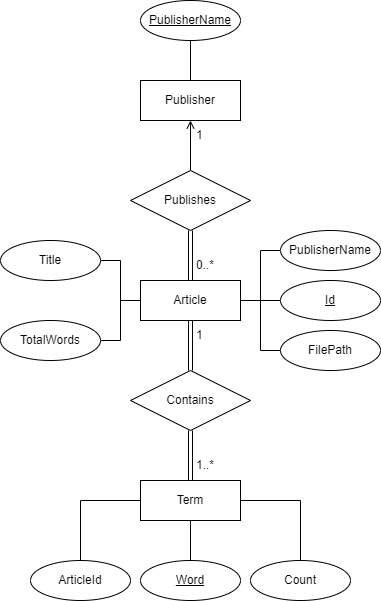
\includegraphics[scale=0.6]{Images/New database model.png}
    \caption{ER diagram of the new database model.}
    \label{newdatabaseER}
\end{figure}

%\vspace{2cm}